% last updated in April 2002 by Antje Endemann
% Based on CVPR 07 and LNCS, with modifications by DAF, AZ and elle, 2008 and AA, 2010, and CC, 2011; TT, 2014; AAS, 2016

\documentclass[runningheads]{llncs}
\usepackage{graphicx}
\usepackage{amsmath,amssymb} % define this before the line numbering.
\usepackage{ruler}
\usepackage{color}
\usepackage[width=122mm,left=12mm,paperwidth=146mm,height=193mm,top=12mm,paperheight=217mm]{geometry}
\begin{document}
% \renewcommand\thelinenumber{\color[rgb]{0.2,0.5,0.8}\normalfont\sffamily\scriptsize\arabic{linenumber}\color[rgb]{0,0,0}}
% \renewcommand\makeLineNumber {\hss\thelinenumber\ \hspace{6mm} \rlap{\hskip\textwidth\ \hspace{6.5mm}\thelinenumber}}
% \linenumbers
\pagestyle{headings}
\mainmatter
\def\ECCV16SubNumber{***}  % Insert your submission number here

\title{Human Emotion Generation with Generative Adversarial Networks} % Replace with your title

\titlerunning{}

\authorrunning{Fan, Y., Liu, S., and Wang, W.}

\author{Yiming Fan, Sicong Liu, Wei Wang}
\institute{KTH Royal Institute of Technology}


\maketitle

\begin{abstract}
We have trained a Generative Adversarial Network (GAN) for generating human faces. This network was inspired from Deep Convolutional GAN (DCGAN) and CycleGAN. Given an arbitrary human face with a certain emotion (e.g.~happy, sad, \dots) we could transform the face into the specified emotion.
\end{abstract}

\section{Introduction \& Related Work}

\subsection{Background: The Uprising of GANs}
Deep Learning (DL) is recently a hot topic in the field of Computer Vision (CV). Some deep networks have reached good performance in the specific areas of image recognition, classification and generation. Among those networks, the Generative Adversarial Network (GAN) excels in extracting, learning and generating features.

Introduced by Goodfellow \cite{goodfellow-2014} in 2014, GAN inspired us with the idea of \textit{MiniMax} training. However the very first generation of GAN remains lots of drawbacks: The difficulty for controlling the step-size of training both the generator and the discriminator and the difficulty for evaluating the performance \cite{arjovsky_bottou_2017}. Therefore a more complete and mature architecture of GAN is necessary.

Up till present there are various variations of GANs published out. For instance: Wasserstein GAN (W-GAN) solves the problems of discrete input function space and the loss of gradients \cite{arjovsky_chintala_bottou_2017}. Deep Convolutional GAN (DCGAN) expands the model complexity and reduces the problems of early-terminating and the hardness to converge \cite{radford_metz_chintala_2016}. The Boundary Equilibrium GAN (BEGAN) provides with an elegant and neat training procedure, and reaches a plausible image generation quality \cite{berthelot_schumm_metz_2017}.

\subsection{Problem Specification}
Our problem aims at generating human faces with specified emotions. Given a digital image containing a face of human, we will have to design a model that could generate a new digital image of the same face, but with any emotion specified. That means we will have to transfer the emotion on the face into arbitrarily specified ones.

\subsection{Dataset}
We choose the Facial Expression Recognition 2013 (\textit{fer2013}) dataset for our problem. It consists of $35887$ gray-scale facial images of $48\times48$ pixels, each of which is labeled with one of seven categories: \textit{angry, disgusted, fearful, happy, sad, surprised} and \textit{neutral}.
\section{Detail of Implementation}
\begin{figure}
\begin{center}
\includegraphics[width=6cm]{./dd2424-pr/2_1.png}
\caption{The overall structure of the network.}
\end{center}
\end{figure}

\subsection{Overall Structure}
The network architecture of the whole network looks similar to what of an \textit{autoencoder} structure but not exactly the same. First we feed the network with a digital image $\textbf{x}$ and a one-hot label $\textbf{y}$ representing any emotion we like. Then $\textbf{x}$ is fed into the encoder $E$ to generate the corresponding stochastic noise $\textbf{z}$:
\begin{equation}
\textbf{z}=E(\textbf{x})
\end{equation}
The architecture of encoder was inspired from the structure in CycleGAN \cite{zhu_park_isola_efros_2017}. It acts like the inverse function of the generator $G$, which could be also considered as the decoder.

After encoding the generated noise $\textbf{z}$ together with the label, $\textbf{y}$ will be sampled through the generator with deep convolutional structure (it was trained within conditional GAN fashion) and we have
\begin{equation}
\textbf{x}^{\prime}=G(\textbf{z}|\textbf{y})
\end{equation}
where $\textbf{x}^{\prime}$ is the generated digital image. We write $G(\cdot|\mathbf{y})$ as the form of conditional probability,\ i.e.~the generalized output given condition $\mathbf{y}$. The generated image $\textbf{x}^{\prime}$ has exactly the same face as what of $\textbf{x}$, but with the emotion labeled as $\textbf{y}$. If $\textbf{y}$ represents the identical emotion as the original image $\textbf{x}$, then $\textbf{x}$ and $\textbf{x}^{\prime}$ will share little or no difference.

We implemented the network based on \texttt{Tensorflow}. Due to some package configuration problems we could not manage to train the network on PDC computers and tried training on persona GPUs instead.

\subsection{Training Procedures}
First we trained the DCGAN within \textit{fer2013} dataset. After successfully training we could generate faces with preset emotions. However we could not yet generate emotions on \textit{arbitrary} human faces. To achieve this we trained $E$. Then by combining the working encoder $E$ with the generator (decoder) $G$ we obtained a completely functioning network which mean the training procedures were done. We will illustrate those procedures below.

\subsubsection*{2.2.1 Training the DCGAN.\ }
\begin{figure}
\begin{center}
\includegraphics[width=12cm]{./dd2424-pr/2_2_1.png}
\caption{The computational graph of the DCGAN.}
\end{center}
\end{figure}
Figure $2$ shows the top architecture of the Deep Convolutional GAN. The only top-level modification to the original GAN is the addition of the conditional variable $\textbf{y}$. In this problem $\textbf{y}$ represents the one-hot label of various emotions hence it has the size of $7\times1$. In the process of \textit{forward pass} $\textbf{y}$ passes the discriminator $D$ and the generator $G$ (which is used during image generation). The discriminator $D$ accepts the generated image $G(\textbf{z})$ from generator $G$. After computing the loss via \texttt{tf.sigmoid\_cross\_entropy\_with\_logits} and \texttt{tf.reduce\_mean}. Finally we sum up the \texttt{D\_loss} and \texttt{G\_loss} respectively and obtain the objective function (similar to those in Conditional GANs \cite{mirza_osindero_2014}):
\begin{equation}
\min\limits_{G}\,\max\limits_{D}V(D,G)=\mathbb{E}_{\textbf{x}}\,(S(D(\textbf{x}|\textbf{y})))+\mathbb{E}_{\textbf{x}}\,(S(1-D(G(\textbf{x}|\textbf{y}))))
\end{equation}
where $D(\cdot)$ represents the output of discriminator $D$, $G(\cdot)$ the output of generator $G$ and $S(\cdot)$ the output of the \texttt{tf.sigmoid\_cross\_entropy\_with\_logits} function:
\begin{equation}
S(\mathbf{x},\mathbf{z})=\mathbf{x}-\mathbf{x}*\mathbf{z}+\log(1+\exp(-\mathbf{x}))
\end{equation}
The loss function of the DCGAN is then:
\begin{align}
L(D)&=\mathbb{E}_{\textbf{x}}\,(S(D(\textbf{x}|\textbf{y}),\,\mathbf{1}(D(\textbf{x}|\textbf{y}))))+\mathbb{E}_{\textbf{x}}\,(S(D(G(\textbf{x}|\textbf{y})),\,\mathbf{0}(D(G(\textbf{x}|\textbf{y}))))\\
L(G)&=\mathbb{E}_{\textbf{x}}\,(S(D(G(\textbf{x}|\textbf{y})),\,\mathbf{1}(D(G(\textbf{x}|\textbf{y}))))
\end{align}
where $\mathbf{1}(\cdot)$ and $\mathbf{0}(\cdot)$ represent the one-like and zero-like matrices respectively. The detailed computational graphs of $D$ and $G$ are shown.
\begin{figure}
\begin{center}
\includegraphics[width=8cm]{./dd2424-pr/2_2_2.png}
\includegraphics[width=8cm]{./dd2424-pr/2_2_3.png}
\caption{The computational graphs of the discriminator $D$ (above) and the generator $G$ (below). \textbf{Explanation on abbreviations}: \texttt{Conv} for 2-dimensional convolution, \texttt{LReLU} for leaky \texttt{ReLU}, \texttt{BN(Conv)} for \textit{Batch Normalization} followed by 2-dimensional convolution, \texttt{FC} for fully-connection, \texttt{DeConv} for 2-dimensional \textit{De-convolution} and \texttt{tanh} for the hyperbolic tangent function.}
\end{center}
\end{figure}

After computing the loss we update the hyper-parameters of $G$ and $D$ by \textit{Adam-optimizer} \cite{kingma_ba_2017} which is an advanced version of the \textit{AdaGrad}. For each timestep $t$ w.r.t.\ each batch of data $\textbf{x}$ we have:
\begin{align}
g_t\,&\leftarrow\,\partial_{\theta}f_t(\theta_{t-1})\\
m_t\,&\leftarrow\,\beta_1\cdot m_{t-1}+(1-\beta_1)\cdot g_t\\
v_t\,&\leftarrow\,\beta_2\cdot v_{t-1}+(1-\beta_2)\cdot g_{t}^{2}\\
\hat{m}_t\,&\leftarrow\,m_t/(1-\beta_{1}^{t})\\
\hat{v}_t\,&\leftarrow\,v_t/(1-\beta_{2}^{t})\\
\theta_t\,&\leftarrow\,\theta_{t-1}-\alpha\cdot\hat{m}_t/(\sqrt{\hat{v}_t}+\epsilon)
\end{align}
where $\theta$ is the hyper-parameter to be updated, $\alpha$ the learning rate, $\beta_1$ and $\beta_2$ the exponential decay rates for the moment estimates, $m$ the first moment vector and $v$ the second moment vector.

By updating hyper-parameters stochastically we will eventually reach the optimum. In practice we may adjust the step-size for training $G$ in order to prevent the early-termination of the discriminator $D$. For ease we may simply change the times of updating $G$ to obtain a suitable step-size.

\subsubsection*{2.2.2 Training the Encoder.\ }
\begin{figure}
\begin{center}
\includegraphics[width=8cm]{./dd2424-pr/2_2_4.png}
\caption{The computational graph of $E$.}
\end{center}
\end{figure}
After training a well functioning generator $G$ we will step forward to train the encoder $E$. The computational graph for $E$ is shown. Similar to what of the discriminator $D$, the \textit{fully-connected} layer of $E$ gives $\mathbf{z}$ as the output instead of a binary value. Given an image $\mathbf{x}$ as the input the encoder will output the stochastic noise $\mathbf{z}$ with the maximum probability such that
\begin{equation}
\mathbf{z}=E(\mathbf{x})=E(G(\mathbf{z}))
\end{equation}
Our aim is to train an encoder that perfectly acts like the `inverse function' of $G$. Therefore the loss function on $E$ is defined as:
\begin{equation}
L(E)=\sum_{\mathbf{x}}\,(\mathbf{x}-G(E(\mathbf{z})))^2
\end{equation}
We will update the hyper-parameters using the same optimizer as above. Only when the network reaches its optimum can we assert the completion of training the whole network.

\subsection{Some Training Notes}
As stated above, we implemented the network within \texttt{Tensorflow}. The hyper-parameters are similar as recommended in \cite{radford_metz_chintala_2016}. The model was trained with stochastic gradient descent (SGD) with a mini-batch of $64$. All weights were initialized as zero-centered normal distribution with standard deviation of $0.02$. The leak slope of leaky \texttt{ReLU} is $0.2$. We used \textit{Adam optimizer} with learning rate of $0.0002$ and momentum $\beta_1$ of $0.5$. The model was trained for $50$ epochs on a \textit{GeForce GTX 1080} graphic card, and the overall elapsed time was around $100$ minutes.

\section{Result of Experiments}
When training the generator $G$, we randomly sampled $64$ points of stochastic noise $\mathbf{Z}$ after training every $100$ batches. With those sampled noise we generated images through $G$.

\begin{figure}
\begin{center}
\includegraphics[width=3.5cm]{./dd2424-pr/train_00.png}
\includegraphics[width=3.5cm]{./dd2424-pr/train_06.png}
\includegraphics[width=3.5cm]{./dd2424-pr/train_12.png}
\includegraphics[width=3.5cm]{./dd2424-pr/train_18.png}
\includegraphics[width=3.5cm]{./dd2424-pr/train_24.png}
\includegraphics[width=3.5cm]{./dd2424-pr/train_39.png}
\caption{Trained pictures after various epochs(from left to right): 0, 6, 12, 18, 24, 39.}
\end{center}
\end{figure}

Figure 5 shows a gallery of sample images after various epochs of training. Looking through the gallery we notice that the generated images with the first few epochs are blurred with lots of noises. This is because neither the generator $G$ nor the discriminator $D$ were sufficiently trained. With the number of epoch increasing we could observe more sampled images being distinguishable and clearer, as hyper-parameters optimized by \textit{Adam optimizer} plateaus.

The sampled images after $24$ and $39$ epochs were having increasingly higher contrasts, which indicated the expanding output range of the \textit{fully-connected} layer. This also indicates the hyper-parameters of $G$ converges to a satisfactory level.

We take $2$ steps for testing the performance of the completely functioning network. First we feed original images (randomly selected from \textit{fer2013}) into the encoder $E$ which produces stochastic noise vectors $\mathbf{z}$. Then we feed $\mathbf{z}$ into $G$ with label $3$, which was supposed to form \textit{happy} emotions from original faces. The outcome could be observed in Figure 6.\newline
\begin{figure}
\begin{center}
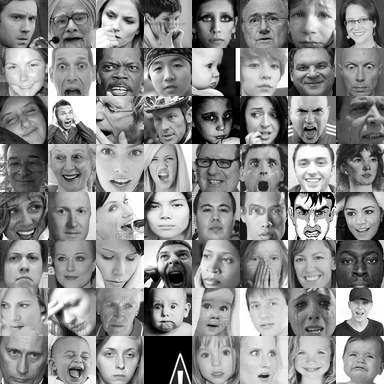
\includegraphics[width=6cm]{./dd2424-pr/test_encoder_original.png}
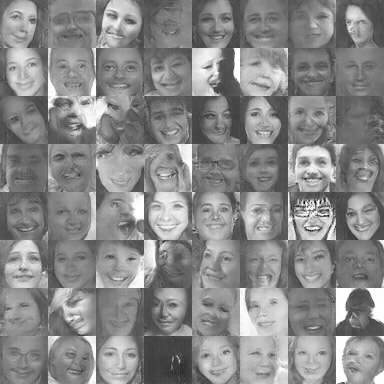
\includegraphics[width=6cm]{./dd2424-pr/test_encoder.png}
\caption{ Original faces and decoded faces }
\end{center}
\end{figure}
The comparison indicates that after decoding, most of the images were transfered into \textit{happy} emotions ``successfully'' with similar outlines and relatively low inaccuracy by intuition. On the other hand, generated images have low contrast after the \textit{fully-connected} layer of generator $G$ which means there were information loss in vectors $\mathbf{z}$ after encoder $E$. 

Moreover, there were some failures upon transferring. Some were due to the wrong storage of datasets such as the fourth images in the last row and others were probably caused by imperfection of encoder $E$ which caused some losses through network, such as the face of \textit{baby} in the second row. Similarly, some pictures were decoded with gender transfer. Taking the first images for instance, the face transfered from male to female, while keeping the outline similar.

Our experiments were not limited to one single emotion. We put original images into $E$ network for generating stochastic noise vectors $\mathbf{z}$. Then they were combined with different labels $\mathbf{y}$ and were taken as input of $G$. Different labels $\mathbf{y}$ (range from $0$ to $6$) could influence outcoming faces, which were shown in Figure $7$. Each cluster of emotions with different labels were compared with those original faces and compared with self-contained meaning as well. Among all generated clusters, there were quite high percentages of face emotions consistent with their own labels. Especially for image clusters with label $3$ and label $5$, almost all images looked ``successful'' to some extent due to both smiling and surprising emotion had unique shapes of mouths whereas other cluster were not so distinguishable but still looked acceptable. 

\begin{figure}
\begin{center}
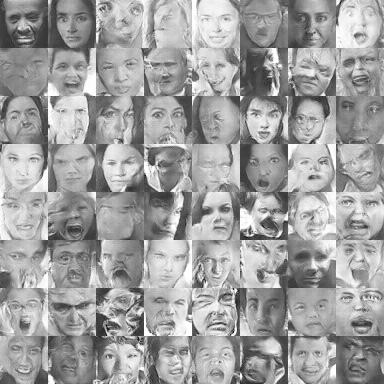
\includegraphics[width=3.5cm]{./dd2424-pr/test_arange_0.png}
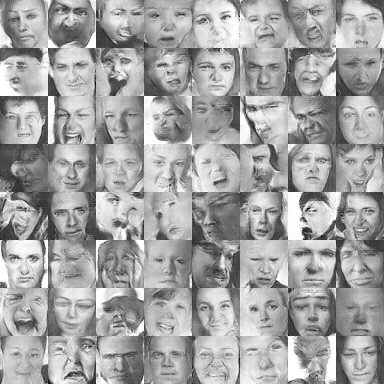
\includegraphics[width=3.5cm]{./dd2424-pr/test_arange_1.png}
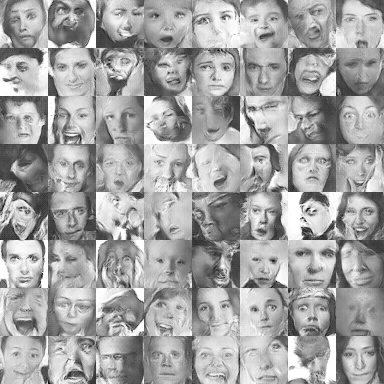
\includegraphics[width=3.5cm]{./dd2424-pr/test_arange_2.png}
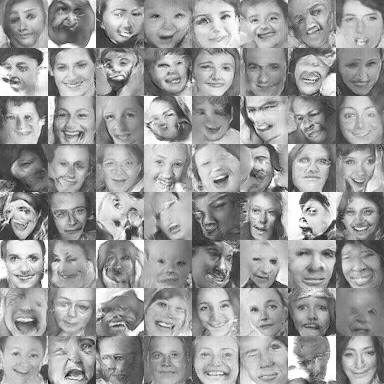
\includegraphics[width=3.5cm]{./dd2424-pr/test_arange_3.png}
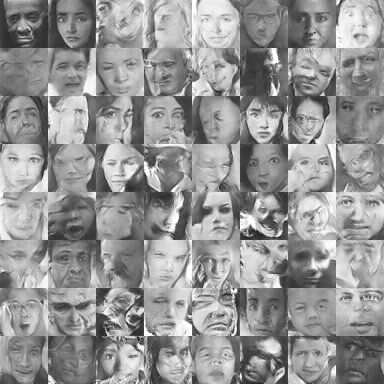
\includegraphics[width=3.5cm]{./dd2424-pr/test_arange_4.png}
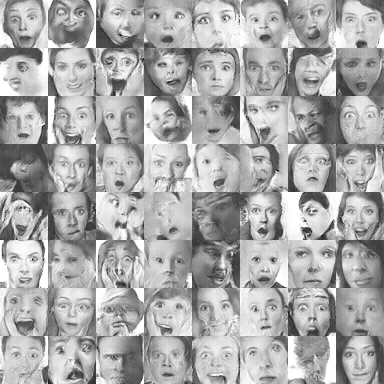
\includegraphics[width=3.5cm]{./dd2424-pr/test_arange_5.png}
\caption{Test pictures with different emotion after decoding: angry, disgusted, fearful, happy, sad, surprised }
\end{center}
\end{figure}

Above results demonstrated that it is easier to train generator by using batch normalization, appropriate activation function and replacing pooling layers with fractional-strided convolutions. With the number of epoch increasing, trained images becomes more distinguishable. It also shows that training encoder with CycleGAN is feasible, regardless some deformed transfer.

\section{Conclusion}

\begin{itemize}
\item We fine-tuned the networks inspired by DCGAN and trained our own dataset \textit{fer2013} which was not conducted identically with \cite{radford_metz_chintala_2016}.
\item We made an extension on training an encoder inspired by CycleGAN and successfully achieved the transfer from encodes (stochastic noise $\mathbf{z}$ generated from $E$) to decodes (image data $\mathbf{x}$ generated from $G$). This encoder together with the Deep Convolutional GAN are encapsulated in the top-level architecture of an \textit{autoencoder}.
\item We achieved \textit{image-to-image style transfer} eventually. The output galleries are imperfect and somehow flawed but satisfactory and acceptable. We consider it a success of our project.
\item The design, implementation and fine-tuning of our project was time-consuming and there remains many uninterpretable points in the latent layers. There remains some weird output images and some are even inhuman. In the future we might improve the network and make a quantity analysis among encoders and decoders. \clearpage
\end{itemize}

\bibliographystyle{splncs}
\bibliography{egbib}
\end{document}
